\documentclass{standalone}
\usepackage{tikz}
\usepackage{amsmath}
\usetikzlibrary{arrows.meta, positioning}
\begin{document}

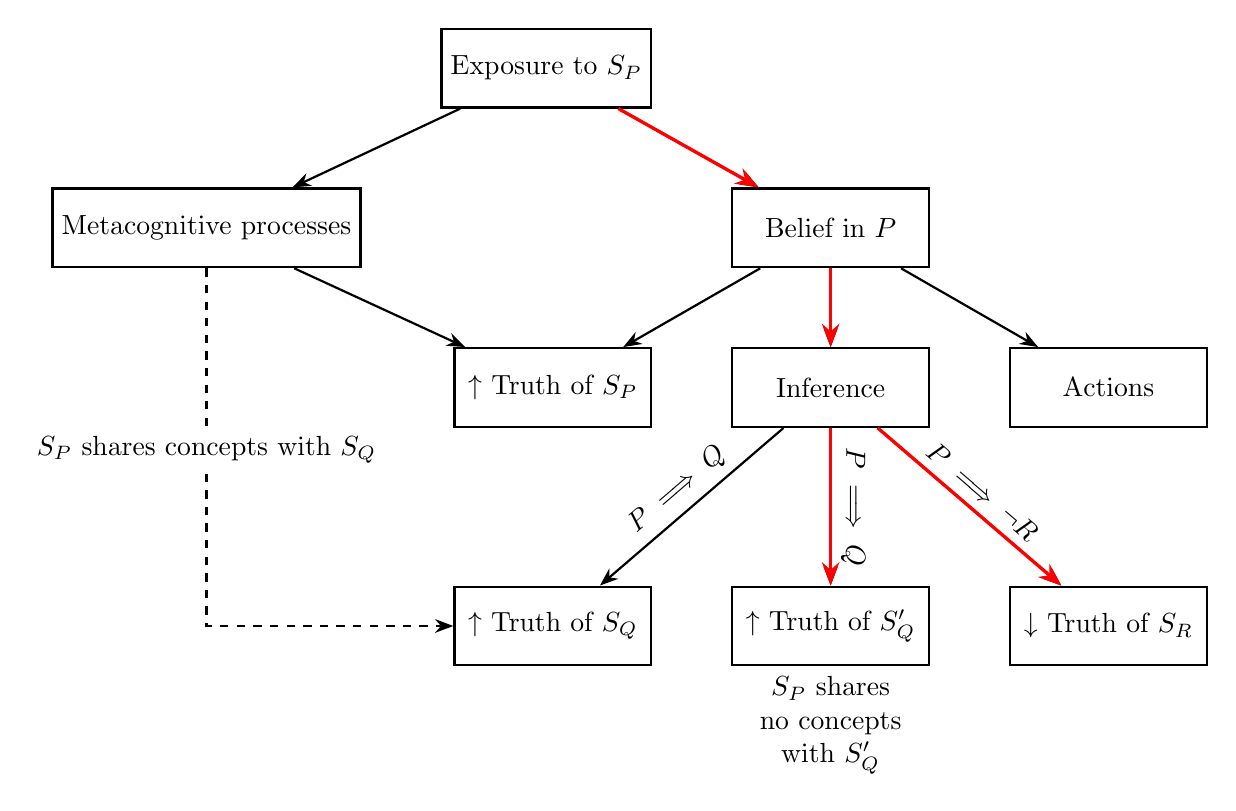
\begin{tikzpicture}[
    squarednode/.style={rectangle, draw=black, thick, minimum height=1cm, minimum width=2.5cm},
    ->, thick, >=Stealth
]

% Nodes
\node[squarednode]      (exposure)                                  {Exposure to $S_P$};
\node[squarednode]      (meta)           [below left=of exposure]   {Metacognitive processes};
\node[squarednode]      (belief)         [below right=of exposure]        {Belief in $P$};
\node[squarednode]      (truthSP)        [below left=of belief]  {$\uparrow$ Truth of $S_P$};
% \node[squarednode]      (concepts)       [below=of meta]            {If $S_P$ shares concepts with $S_Q$};
\node[squarednode]      (inference)      [below=of belief]          {Inference};
\node[squarednode]      (actions)        [below right=of belief]    {Actions};
\node[squarednode]      (truthSQ)        [below left=of inference, yshift=-1cm]          {$\uparrow$ Truth of $S_Q$};
\node[squarednode]      (truthSQprime)   [below=of inference, yshift=-1cm]         {$\uparrow$ Truth of $S'_Q$};
\node[squarednode]      (truthSR)        [below right=of inference, yshift=-1cm]       {$\downarrow$ Truth of $S_R$};
\node[draw=none,fill=none]      (concepts)   [below=of meta, yshift=-1cm]  {$S_P$ shares concepts with $S_Q$};
\node[draw=none, fill=none, text width=2.54cm,align=center]      (Noconcepts)   [below=of truthSQprime, yshift=1cm]  {$S_P$ shares no concepts with $S'_Q$};

% Arrows
\draw[->] (exposure) -- (meta);
% \draw[->] (exposure.south) -- (truthSP.north);
\draw[->] (exposure) -- (belief);
\draw[red, very thick] (exposure) -- (belief);
\draw[->] (belief) -- (actions);
\draw[->] (meta) -- (truthSP);
% \draw[->] (meta.south) -- (concepts.north);
% \draw[dashed, ->] (concepts.east) -- (truthSQ.west);
\draw[dashed, -] (meta) -- (concepts);
% \draw[dashed, |->] (concepts) -- (truthSQ.west);
\draw[dashed, ->] (concepts.south) |- (truthSQ.west);
\draw[->] (belief) -- (truthSP);
\draw[->] (belief) -- (inference);

\draw[red, very thick] (belief) -- (inference);
% \draw[->] (inference) -- (truthSR);
\draw[->] (inference)  -- (truthSR) node [midway, above, sloped] (TextNode) {$P \implies \neg R$};
\draw[red, very thick] (inference)  -- (truthSR);
\draw[->] (inference) -- (truthSQ) node [midway, above, sloped] (TextNode) {$P \implies Q$};
\draw[->] (inference) -- (truthSQprime) node [midway, above, sloped] (TextNode) {$P \implies Q$};
\draw[red, very thick] (inference) -- (truthSQprime);

\end{tikzpicture}

\end{document}
